%
% Rewriting Open Graphs
%

\documentclass{amsart}
%
%	rewriting open objects
%	style
%	


%
%  packages
%

\usepackage{amsfonts}
\usepackage{amssymb}  
\usepackage{amsthm} 
\usepackage{amsmath} 
\usepackage{caption}
\usepackage[inline]{enumitem}
	\setlist{itemsep=0em, topsep=0em, parsep=0em}
	\setlist[enumerate]{label=(\alph*)}
\usepackage{doi}
\usepackage{etoolbox}
\usepackage[]{hyperref}
%	\definecolor{hyperrefcolor}{rgb}{0,0,0.7}
	\hypersetup{colorlinks,linkcolor={blue},citecolor={blue},urlcolor={blue}}
\usepackage{graphicx}
\usepackage{mathtools}
\usepackage[numbers]{natbib}
\usepackage{stmaryrd} 
\usepackage{subcaption}
\usepackage{subfiles}
\usepackage{tikz}
	\usetikzlibrary{matrix,arrows,shapes,decorations.markings,decorations.pathreplacing}
\usepackage{todonotes}
\usepackage{url}
\usepackage{xcolor}

%
% commands
%

\newcommand{\RR}{\mathbb{R}}
\newcommand{\ZZ}{\mathbb{Z}}
\newcommand{\NN}{\mathbb{N}}
\newcommand{\QQ}{\mathbb{Q}}
\newcommand{\CC}{\mathbb{C}}
\newcommand{\DD}{\mathbb{D}}
\newcommand{\MM}{\mathbb{M}}
\renewcommand{\epsilon}{\varepsilon}

\newcommand{\Set}{\cat{Set}}
\newcommand{\Graph}{\cat{Graph}}
\newcommand{\RGraph}{\cat{RGraph}}
\newcommand{\Top}{\cat{Top}}
\newcommand{\Cat}{\cat{Cat}}
\newcommand{\A}{\cat{A}}
\newcommand{\B}{\cat{B}}
\newcommand{\C}{\cat{C}}
\newcommand{\X}{\cat{X}}
\newcommand{\Y}{\cat{Y}}
\newcommand{\Z}{\cat{Z}}
\newcommand{\core}[1]{\mathbf{core}(#1)}

\newcommand{\defn}[1]{\textbf{#1}}
\newcommand{\op}[1]{\operatorname{#1}}
\newcommand{\cat}[1]{\mathbf{#1}}
\newcommand{\dblcat}[1]{\mathbb{#1}}
\renewcommand{\t}[1]{\text{#1}}


\newcommand{\from}{\colon}
\newcommand{\xto}[1]{\xrightarrow{#1}}
\newcommand{\sm}{\smallsetminus}
\newcommand{\tospan}{\xrightarrow{\mathit{sp}}}
\newcommand{\tocospan}{\xrightarrow{\mathit{csp}}}
\newcommand{\diagram}[1]{\raisebox{-0.5\height}{\includegraphics{#1}}}

\newcommand{\Sp}[1]{\mathbf{Sp}(#1)}
\newcommand{\MonSp}[1]{\mathbf{MonSp}(#1)}
\newcommand{\SSp}[1]{\mathbb{S}\mathbf{p}(#1)}
\newcommand{\Csp}[1]{\mathbf{Csp}(#1)}
\newcommand{\CCsp}[1]{\mathbb{C}\mathbf{sp}(#1)}
\newcommand{\SpSp}[1]{\mathbf{Sp}(\mathbf{Sp}(#1))}
\newcommand{\SSpSp}[1]{\mathbb{S}\mathbf{p(\mathbf{Sp}(#1))}}
\newcommand{\CspCsp}[1]{\mathbf{Csp}(\mathbf{Csp}(#1))}
\newcommand{\CCspCsp}[1]{\mathbb{C}\mathbf{sp}(\mathbf{Csp}(#1))}
\newcommand{\MonSpCsp}[1]{\mathbf{MonicSp}(\mathbf{Csp}(#1))}
\newcommand{\MMonSpCsp}[1]{\mathbb{M}\mathbf{onicSp}(\mathbf{Csp}(#1))}
\newcommand{\EpCspSp}[1]{\mathbf{EpicCsp}(\mathbf{Csp}(#1))}
\newcommand{\EEpCspSp}[1]{\mathbb{E}\mathbf{picCsp}(\mathbf{Sp}(#1))}
\newcommand{\SpCsp}[1]{\mathbf{Sp}(\mathbf{Csp}(#1))}
\newcommand{\SSpCsp}[1]{\mathbb{S}\mathbf{p}(\mathbf{Csp}(#1))}

\newcommand{\FuncCsp}[1]{ #1 \t{-} \mathbf{Csp}}
\newcommand{\OpenOb}[1]{ #1 \t{-} \mathbf{Open} }
\newcommand{\Rewrite}[1]{ #1 \t{-} \mathbf{Rewrite} }
\newcommand{\RRewrite}[1]{ #1 \t{-} \mathbb{R}\mathbf{ewrite} }
\newcommand{\MonRewrite}[1]{ #1 \t{-} \mathbf{MonRewrite} }
\newcommand{\MMonRewrite}[1]{ #1 \t{-} \mathbb{M}\mathbf{on}\mathbb{R}\mathbf{ewrite} }

%
% math operators
%

\DeclareMathOperator{\Hom}{Hom}
\DeclareMathOperator{\id}{id}
\DeclareMathOperator{\ob}{Ob}
\DeclareMathOperator{\arr}{arr}
\DeclareMathOperator{\im}{im}
\DeclareMathOperator{\Aut}{Aut}
\DeclareMathOperator{\Bij}{Bij}
\DeclareMathOperator{\Sub}{Sub}
\DeclareMathOperator{\colim}{colim}

%
% envirnments and counters
%

\newtheorem{thm}{Theorem}[section]
\newtheorem{lem}[thm]{Lemma}
\newtheorem{prop}[thm]{Proposition}
\newtheorem{cor}[thm]{Corollary}

\theoremstyle{remark}
	\newtheorem{remark}[thm]{Remark}
	\newtheorem{notation}[thm]{Notation}

\theoremstyle{definition}
	\newtheorem{ex}[thm]{Example} 
	\newtheorem{df}[thm]{Definition}

% \setcounter{tocdepth}{1} % Sets depth for table of contents. 

%
% tikz types
%

\tikzset{->-/.style={decoration={%
			markings,
			mark=at position .5 with {\arrow{>}}},postaction={decorate}}
}
\tikzset{->-pos/.style={decoration={%
			markings,
			mark=at position #1 with {\arrow{>}}},postaction={decorate}}
}
\tikzset{->-/.style={decoration={%
			markings,
			mark=at position .5 with {\arrow{>}}},postaction={decorate}}
}
\tikzset{->-pos/.style={decoration={%
			markings,
			mark=at position #1 with {\arrow{>}}},postaction={decorate}}
}
 

\begin{document} % document
\begin{abstract} % abstract
	open graphs, 
	their rewrites, 
	and an application
\end{abstract}	

\title{Rewriting open graphs}
\author{Daniel Cicala}
\maketitle

\section{Introduction} % intro

%_______begin intro

Our goal is to model open networks 
and their rewrites.  By an \emph{open network},
we mean a network together with a boundary.
To make this precise, we
begin with a category of `input and output types' 
$\cat{C}$
and another category of `networks' 
$ \cat{D} $.
To equip a network, an object of $\cat{D}$,
with a boundary, a pair of objects from $\cat{C}$,
we use an adjunction
\[ % adjoint diagram
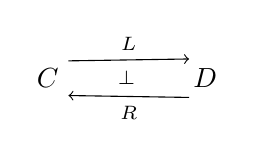
\begin{tikzpicture} 
\node (C) at (0,0) {$ C $};
\node (D) at (2,0) {$ D $};
\node at (1,0) {\scriptsize $ \perp $};
\draw [->] (C.40) to 
node [above] {\scriptsize $ L $} (D.130);
\draw [<-] (C.-40) to 
node [below] {\scriptsize $ R $} (D.-130);
\end{tikzpicture}
\]
With this setup, we focus on three categories.

The first category, denoted 
$ \LspanD $,
has as objects, those from $ \cat{C} $,
and as arrows, cospans of the form
\[
Lc \to d \gets Lc'
\]
inside of $ \cat{D} $.

The second category, denoted
$ \LopenD $,
has cospans
\[
Lc \to d \gets Lc'
\]
in $ \cat{ D } $ for objects and
triples of arrows $ ( f , g , h ) $
such that 
\[  % diagram for L-open arrows  
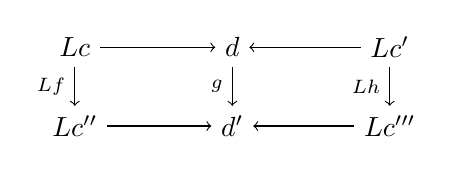
\begin{tikzpicture}
\node (Lc) at (-2,1) {$ Lc $};
\node (d) at (0,1) {$ d $};
\node (Lc') at (2,1) {$ Lc' $};
\node (Lc'') at (-2,0) {$ Lc'' $};
\node (d') at (0,0) {$ d' $};
\node (Lc''') at (2,0) {$ Lc''' $};
\draw [->] (Lc) to (d);
\draw [->] (Lc') to (d);
\draw [->] (Lc'') to (d');
\draw [->] (Lc''') to (d');
\draw [->] (Lc) to node [left] {\scriptsize $ Lf $ } (Lc'');
\draw [->] (d) to node [left] { \scriptsize $ g $ }(d');
\draw [->] (Lc') to node [left] { \scriptsize $ Lh $ }(Lc''');
\end{tikzpicture}
\]
commutes.
We show that, when $ \cat{C} $ and
$ \cat{D} $ are topoi, then so is $ \LopenD $.

The third category, denoted
$ \LrewriteD $,
again has cospans 
\[
Lc \to d \gets Lc'
\]
in $ \cat{D} $ for objects and
\emph{cubical spans of cospans}, that is
commuting diagrams 
\[ % cubical span of cospans
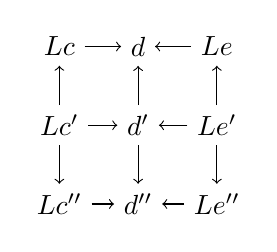
\begin{tikzpicture}
\node (Lc) at (-1,1) {$ Lc $};
\node (Lc') at (-1,0) {$ Lc' $};
\node (Lc'') at (-1,-1) {$ Lc'' $};
\node (d) at (0,1) {$ d $};
\node (d') at (0,0) {$ d' $};
\node (d'') at (0,-1) {$ d'' $};
\node (Le) at (1,1) {$ Le $};
\node (Le') at (1,0) {$ Le' $};
\node (Le'') at (1,-1) {$ Le'' $};
\draw [->] (Lc) to (d);
\draw [->] (Le) to (d);
\draw [->] (Lc') to (d');
\draw [->] (Le') to (d');
\draw [->] (Lc'') to (d'');
\draw [->] (Le'') to (d'');
\draw [->] (Lc') to (Lc);
\draw [->] (Lc') to (Lc'');
\draw [->] (d') to (d);
\draw [->] (d') to (d'');
\draw [->] (Le') to (Le);
\draw [->] (Le') to (Le'');
\end{tikzpicture}
\]
for arrows.  

How do these three categories help
us to model open networks?
To answer this, we first make the
observation that cospans of the form
\[
Lc \to d \gets Lc'
\]
have showed up in each of the above
categories. We call such cospans
\emph{$L$-open objects}.  The term ``open''
indicates that we are thinking of $d$ as 
an object that can `interact' with certain 
elements. More concretely, we say that $ d $ 
has inputs $Lc$ and outputs $ Lc' $ which allow
$ d $ to be glued together with any other
$ L $-open object with outputs $ Lc $ or 
inputs $ Lc' $.  This would give us a zig-zag
which we turn into an $ L $-open object
via pushout.  But this is exactly the composition
in $ \LspanD $. Hence, through their `openness' 
we can think of $ L $-open objects as arrows.
This is not the only perspective we take, however.

Through the categories $ \LopenD $ and $ \LrewriteD $,
we can think of $ L $-open objects as, well, objects.
Certainly, the arrows of $ \LopenD $ are the best
candidate for a morphism of $ L $-open objects.  
We show that $ \LopenD $ is actually a topos.
Then, by work of Lack and Sobocinski, we know that
$ L $-open objects admit a nice (double pushout)
rewriting theory. The sort of rewriting theory we are
interested in, and that Lack and Sobocinski study,
uses spans 
\[
\ell \to k \gets r
\]
to say that the object $ \ell $ is
rewritten to the object $ r $, where $ k $
is some interface common to both 
$ \ell $ and $ r $.  Translating this to the topos 
$ \LopenD $, we consider spans of $ L $-open objects
which are exactly the arrows for $ \LrewriteD $.
Therefore, we think of $ \LopenD $ as the
category of $ L $-open objects with their
morphisms and $ \LrewriteD $ as the category
of $ L $-open objects and their rewrite rules.  

HERES A CHANGE

%_______end intro

\section{Bibliography} % biblio
\bibliographystyle{abbrvnat}
\bibliography{reopn_biblio.bib}
	
\end{document}